\documentclass[11pt,a5paper]{article}

\usepackage[T1]{fontenc} % font encoding, lubab õ tähte kasutada
\usepackage[utf8]{inputenc} % oleme siiski 21. sajandis, vajadusel on ka olemas utf8x
\usepackage{lmodern} % lmodern ja micrtype käivad käsikäes, teeb teksti ilusamaks
\usepackage{microtype}
\usepackage[estonian]{babel} % eesti keele poolitamisreeglid jpm
\usepackage[per = fraction, expproduct=cdot, decimalsymbol=comma, inter-unit-product=\cdot]{siunitx} % http://www.bakoma-tex.com/doc/latex/siunitx/siunitx.pdf
\usepackage{graphicx}
\usepackage{wrapfig}
\usepackage{tikz}
\usepackage[european]{circuitikz}
\tikzset{component/.style={draw,thick,circle,fill=white,minimum size =0.75cm,inner sep=0pt}}
\usepackage{amsmath,amssymb}
\usepackage{amsfonts}
\usepackage{epstopdf} %minul on vaja, et .eps pilte saada
\usepackage{enumitem}
%paneme kõik mõõdud paika
\topmargin=-3.0cm \textheight=19cm \textwidth=12.9cm
\oddsidemargin=-1.5cm  \evensidemargin=-1.5cm
\setlength{\parindent}{0pt} \setlength{\parskip}{6pt} \sloppy
\relpenalty=10000 \binoppenalty=10000 % Tekstisisestes valemites reavahetusi ärgu olgu
\pagestyle{empty} % ilma leheküljenumbrita
\newcommand{\numb}[1]{\vspace{5pt}\textbf{\large #1}}
\newcommand{\nimi}[1]{(\textsl{\small #1})}
\newcommand{\punktid}[1]{(\emph{#1~p.})}
\newcounter{ylesanne}
\newcommand{\yl}[1]{\addtocounter{ylesanne}{1}\numb{\theylesanne.} \nimi{#1} \newblock{}}
\newcommand{\autor}[1]{\emph{ Autor: #1}}
\newcommand{\D}{\textrm{d}}

\begin{document}

\begin{center}
\textbf{\Large Eesti koolinoorte 67. füüsikaolümpiaad} \vspace{3pt}

\emph{9. juuni 2020. a. Lõppvoor.}

\emph{Gümnaasiumi ülesanded (10. - 12. klass)}

\emph{Palun kirjutage iga ülesande lahendus eraldi lehele!}

\end{center}

\yl{KLAASKERA}
Taskulambiga, millest väljuva valgusvihu läbimõõt on $d$, valgustatakse suurt
klaasist kera läbimõõduga $D$. Milline peaks olema klaasi murdumisnäitaja, et
valgusvihk kera keskpunkti suunates koonduks klaaskera pinnal? Eeldada, et
valgusvihu diameeter on tunduvalt väikesem kera läbimõõdust ($d\ll D$) ning et
taskulambist väljuv valgusvihk on paralleelne.
\punktid{6}

\emph{Vihje:} Väikeste nurkade korral $\sin \alpha \approx \alpha$, kui $\alpha$
on radiaanides.

\yl{KOHUKESED}
Richard ostis kohukesi, mis on ühtlase kihina poekoti põhjas. Heatujulisena teeb
ta kotiga vertikaalseid ringe, aga siis hakkab kohukeste pärast muretsema. Õnneks
selgub, et need ei kukkunud välja ja lömaks ka ei läinud. Näidake, et kui Richard
kotiga ei vehi (ega seda keeruta), siis võib ta panna koti põhja kaks korda
paksema kihi kohukesi, ilma et ükski kohuke lömastuks. Kohukesi võib käsitleda
vedelikuna. Võib eeldada, et kohuke lömastub siis, kui rõhk tema juures ületab
mingi kriitilise väärtuse. Vertikaalsete ringide tegemisel on Richardi käe
nurkkiirus konstantne. Eeldada, et kohukeste kihi paksus on palju väiksem kui
ringi raadius.
\punktid{8}

\begin{wrapfigure}{r}{0.35\textwidth}
  \vspace{-25pt}
  \begin{center}
  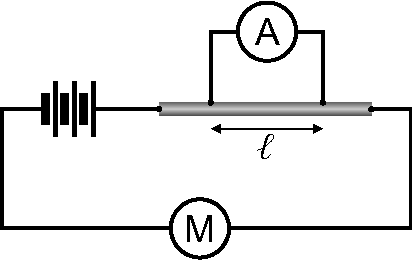
\includegraphics[scale=0.6]{kaivitusvool_joonis.pdf}
  \vspace{-20pt}
  \end{center}
\end{wrapfigure}
\yl{KÄIVITUSVOOL}
Taavet otsustas ära mõõta auto käivitusvoolu tugevuse. Ta leidis ampermeetri
mõõtepiirkonnaga~$I_0=\SI{1}{\milli\ampere}$ ja sisetakistusega~$R_0=\SI{100}{\ohm}$
ja paraja pikkusega jupi vasktoru, mille sisediameeter oli
$d_1=\SI{6}{\milli\meter}$ ja välisdiameeter $d_2=\SI{8}{\milli\meter}$. Ta ühendas
vasktoru jadamisi autoaku ja starteriga (mida võib käsitleda kui takistit) ning ampermeetri rööbiti
vasktoruga nagu kujutatud kõrvaloleval skeemil. Milline tuleks
valida kontaktide vaheline distants~$\ell$, et ampermeetri maksimaalsele
näidule~$I_0$ vastaks mõõdetava voolu suurus $I_1=\SI{500}{\ampere}$?
Vase eritakistus on $\rho=\SI{1.68e-8}{\ohm\meter}$. Ühendusjuhtmete ja
-kontaktide takistused võib lugeda tühiseks.
\punktid{8}

\newpage
\begin{wrapfigure}{r}{0.35\textwidth}
  \vspace{-5pt}
  \begin{center}
  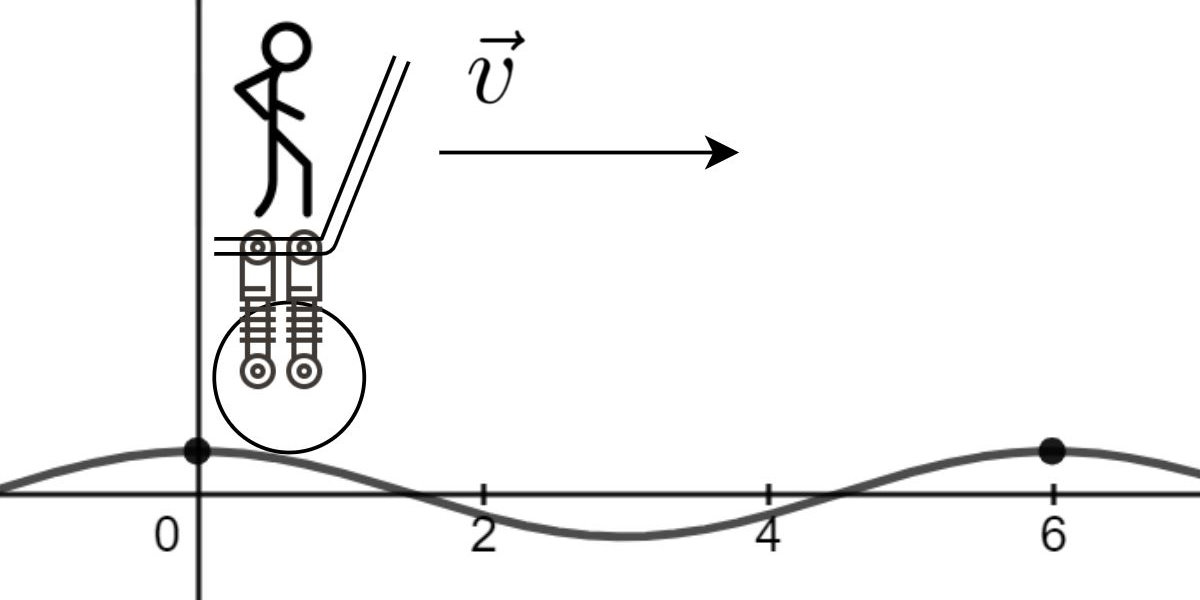
\includegraphics[scale=0.1]{tasakaaluliikur.png}
  \end{center}
  \vspace{-25pt}
\end{wrapfigure}
\yl{TASAKAALULIIKUR}
Hannes massiga $m = \SI{75}{\kilo\gram}$ sõidab tasakaaluliikuriga  konarlikul
teel ühtlase kiirusega $v$. Konarliku tee profiili saab külgvaates lähendada
koosinuslainele amplituudiga~$A = \SI{60}{\milli\meter}$ ja
perioodiga~$\Delta x = \SI{6}{\meter}$. Tasakaaluliikuril on amortiseerimissüsteem,
mis koosneb $n=2$ rööbiti ühendatud vedrust jäikusega $k = \SI{900}{\newton\per\meter}$.
Leidke kiirus~$v$, mille juures Hannes võngub enim ehk tekib resonants.
Tasakaaluliikuri kaal on tühine. Kiirus $v$ on kiirus, mida näitaks
tasakaaluliikuril olev GPS seade, mitte ratta keerlemisel põhinev odomeeter.
\punktid{8}

\emph{Vihje:} Kui keha kiirendus $a$ ja kaugus tasakaalupunktist $y$ on seotud
võrdusega $a=-\omega^2 y$, kus $\omega$ on positiivne konstant, siis võngub keha
perioodiga~$\frac{2\pi}{\omega}$.

\begin{wrapfigure}{r}{0.35\textwidth}
  \vspace{-25pt}
  \begin{center}
  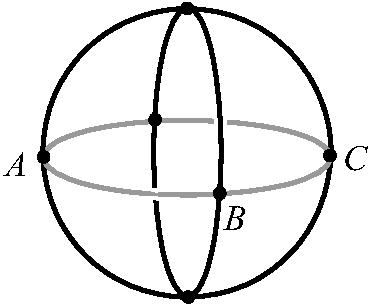
\includegraphics[scale=0.7]{Gloobus_joonis.pdf}
  \end{center}
  \vspace{-25pt}
\end{wrapfigure}
\yl{GLOOBUS}
Sandral oli igav ja ta leidis vanatädi sahtlist kolm traadijuppi.
Ta ühendas need võrdsete raadiustega rõngasteks ning ehitas  huvi pärast gloobuse,
nii nagu joonisel näidatud. Rõngad jaotasid üksteist võrdselt neljaks ning nende
lõikepunktides olid sõlmed. Traadid olid ühtlase joontakistusega ning Sandra mõõtis
oommeetriga üksikute traadijuppide takistusteks $R_1=\SI{4}\Omega$ (joonisel hall
rõngas) ja $R_2=\SI{8}\Omega$ (joonisel mustad rõngad). Mis oleks mõõdetav takistus \\
\osa~klemmide \emph{A} ja \emph{C} vahel;\\
\osa~klemmide \emph{A} ja \emph{B} vahel.\\
\punktid{10}

\yl{PALLIVISKENÕLV}
Oleg viskab jalgpalliväljaku otsajoone tagant väljakule palli. Selgub, et sealt
jaksab ta visata maksimaalselt väljaku keskjooneni, mis asub kaugusel $L$. Ta
tahab ehitada otsajoone taha sellise nõlva, mille igast punktist jaksaks ta visata
maksimaalselt väljaku keskjooneni. Milline peaks olema selle nõlva kõrgusprofiil?

Võib eeldada, et maksimaalne kiirus, millega Oleg suudab palli visata, ei sõltu
viskamissuunast. Õhutakistust võib ignoreerida. Vastuse võib anda kujul $y=f(x)$
või $x=g(y)$.
\punktid{10}

\newpage

\begin{wrapfigure}{r}{0.35\textwidth}
  \vspace{-8pt}
  \begin{center}
  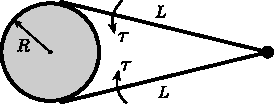
\includegraphics[scale=0.9]{pulgad_joon.pdf}
  \end{center}
  \vspace{-25pt}
\end{wrapfigure}
\yl{PULGAD}
Kaks pulka pikkusega $L$ on otsapidi kinnitatud hõõrdevaba kinnitusega.
Hõõrdevabal horisontaalsel laual on silinder raadiusega $R$ ja massiga $m$.
Joonisel on kujutatud silinder ja pulgad pealtvaates. Eeldame, et pulki hoitakse
alati horisontaalselt nagu joonisel, nendega haaratakse kinni silindri keskelt,
pulkade otsad on täpselt silindri puutepunktides ning pulkade mass on tühine.
Samuti eeldame, et silindri massikese on puutepunkte ühendava lõigu keskpunktis.\\
\osa Leidke minimaalne hõõrdetegur $\mu_{\min}$ pulkade ja silindri vahel,
et silindrist pulkade abil kinni haarates see pulkade vahelt ära ei libiseks.\\
\osa Olgu hõõrdetegur pulkade ja silindri vahel $\mu > \mu_{\min}$. Leidke
minimaalne vajalik jõumoment $\tau_{\min}$, mida tuleb pulkadele avaldada, et
silindrist pulkade abil kinni haarates oleks võimalik silinder laualt üles
tõsta. Maa raskuskiirendus on $g$.
\punktid{12}

\begin{wrapfigure}{r}{0.35\textwidth}
  \vspace{-25pt}
  \begin{center}
  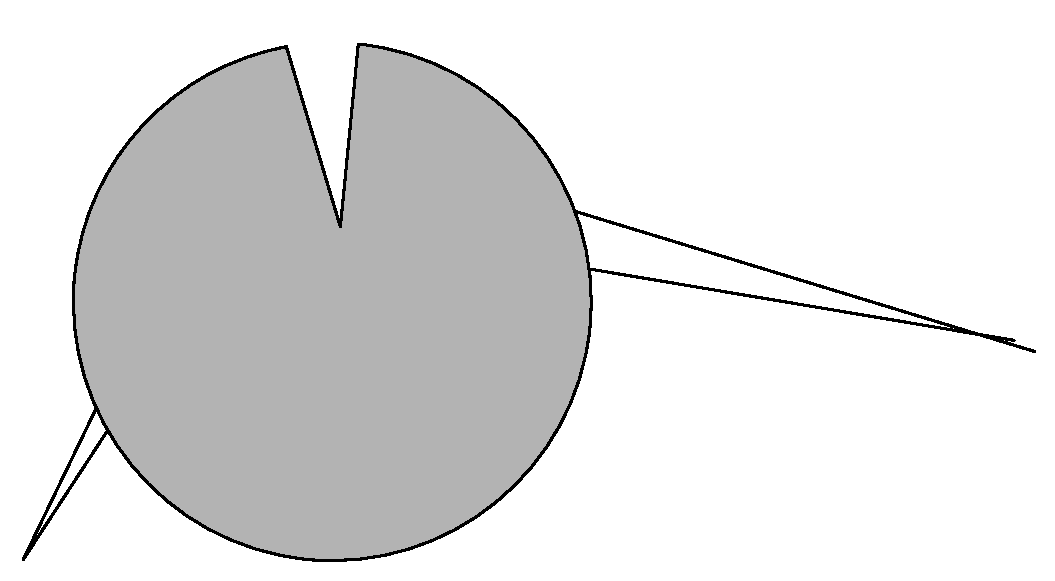
\includegraphics[scale=0.25]{optiline-silinder.pdf}
  \end{center}
  \vspace{-25pt}
\end{wrapfigure}
\yl{OPTILINE SEADE}
Kiilukujulise sisselõikega silindri sees on kaks üksteisega paralleelset peeglit,
mis on paralleelsed ka silindri teljega. Valguskiired saavad silindrisse siseneda
ja sealt väljuda läbi silindri seintes olevate aukude. Silinder on seest õõnes
ning selle seinad on mittepeegeldavad. Joonisel on kujutatud
silinder pealtvaates koos kahe silindrisse siseneva ning peale peegeldusi sealt
väljuva kiirega. Rekonstrueerige peeglite asukohad ning kiirte käik (leidke
vähemalt üks võimalik lahendus). Lahendus esitage lisalehel.
\punktid{12}

\yl{ÕHUPALLID}
Kaur otsustas vaakumkambris kahe õhupalliga eksperimenti teha. Alustuseks ühendas
ta mõlemad õhupallid toruga, mille keskel asus ventiil. Hoides ventiili suletuna,
lasi ta mõlemasse õhupalli sama hulga õhku. Kuna õhupallid olid tehtud erinevatest
materjalidest, paisusid nad erineval määral. Esimene õhupall paisus peale pika aja
möödumist raadiuseni~$r_1$ ning teine raadiuseni~$r_2$, kusjuures $r_1 > r_2$.
Seejärel avas ta ventiili ning lasi õhul vabalt ühest õhupallist teise liikuda.
Missugused on mõlema õhupalli uued raadiused, $R_1$ ja $R_2$, peale pika aja
möödumist? Pika aja möödumisel saavad õhupallide temperatuurid võrdseks
välistemperatuuriga (musta keha kiirguse kaudu). Eeldada, et torus oleva õhu
ruumala on tühine võrreldes õhupallide ruumalaga ning et õhupallid on ideaalsed
kerad. Õhupallide kesti võib lugeda hüperelastseteks materjalideks, mis alluvad
lineaarsele elastsusmudelile $\sigma = E\epsilon$, kus $\sigma$ on materjali pinge
pindalaühiku kohta, $E$ materjali Youngi moodul ning $\epsilon = \Delta L / L_0$
materjali moone. Õhupallide puhul võib eeldada et deformatsioon on algsest
pikkusest palju suurem, s.t. $\Delta L \gg L_0$. Lisaks eeldada, et paisumise
käigus jääb õhupallide kesta ruumala samaks ning et kesta paksus on õhupalli
lineaarmõõtmega võrreldes tühine.
\punktid{12}


\begin{wrapfigure}{r}{0.35\textwidth}
  \vspace{-25pt}
  \begin{center}
  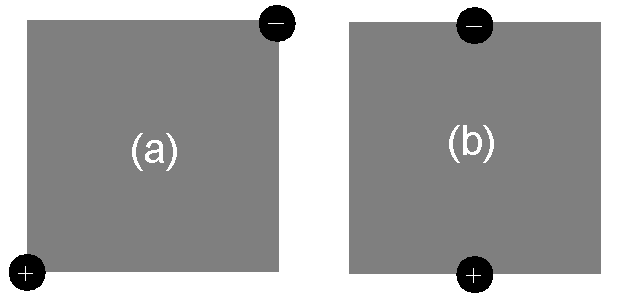
\includegraphics[scale=0.44]{kauri-ruut.pdf}
  \end{center}
  \vspace{-25pt}
\end{wrapfigure}
\yl{RUUT}
Ühtlase takistusega ruudust plaadi vastastippude vaheliseks takistuseks mõõdetakse
$R$, vt joonis (a). Milline tulemus saadakse sama ruudu vastaskülgede keskpunktide
vahelise takistuse mõõtmisel, vt joonis (b)? Mõlemal juhul kasutatakse oommeetri
ühendamiseks samu kettakujulisi tühise takistusega elektroode, mis surutakse vastu
plaati nii nagu näidatud joonisel.
\punktid{14}

\end{document}
